\chapter{Конструкторский раздел}

\section{Логическое проектирование базы данных}\label{sec:db-design}

Схема базы данных (рисунок~\ref{fig:relational-schema}) включает восемь
таблиц. Факты хранятся в \newline \texttt{game\_player\_stats}, денормализованная
витрина \texttt{player\_season\_stats} ускоряет аналитические выборки.
Справочники используют суррогатные ключи.

\begin{figure}[H]
\centering
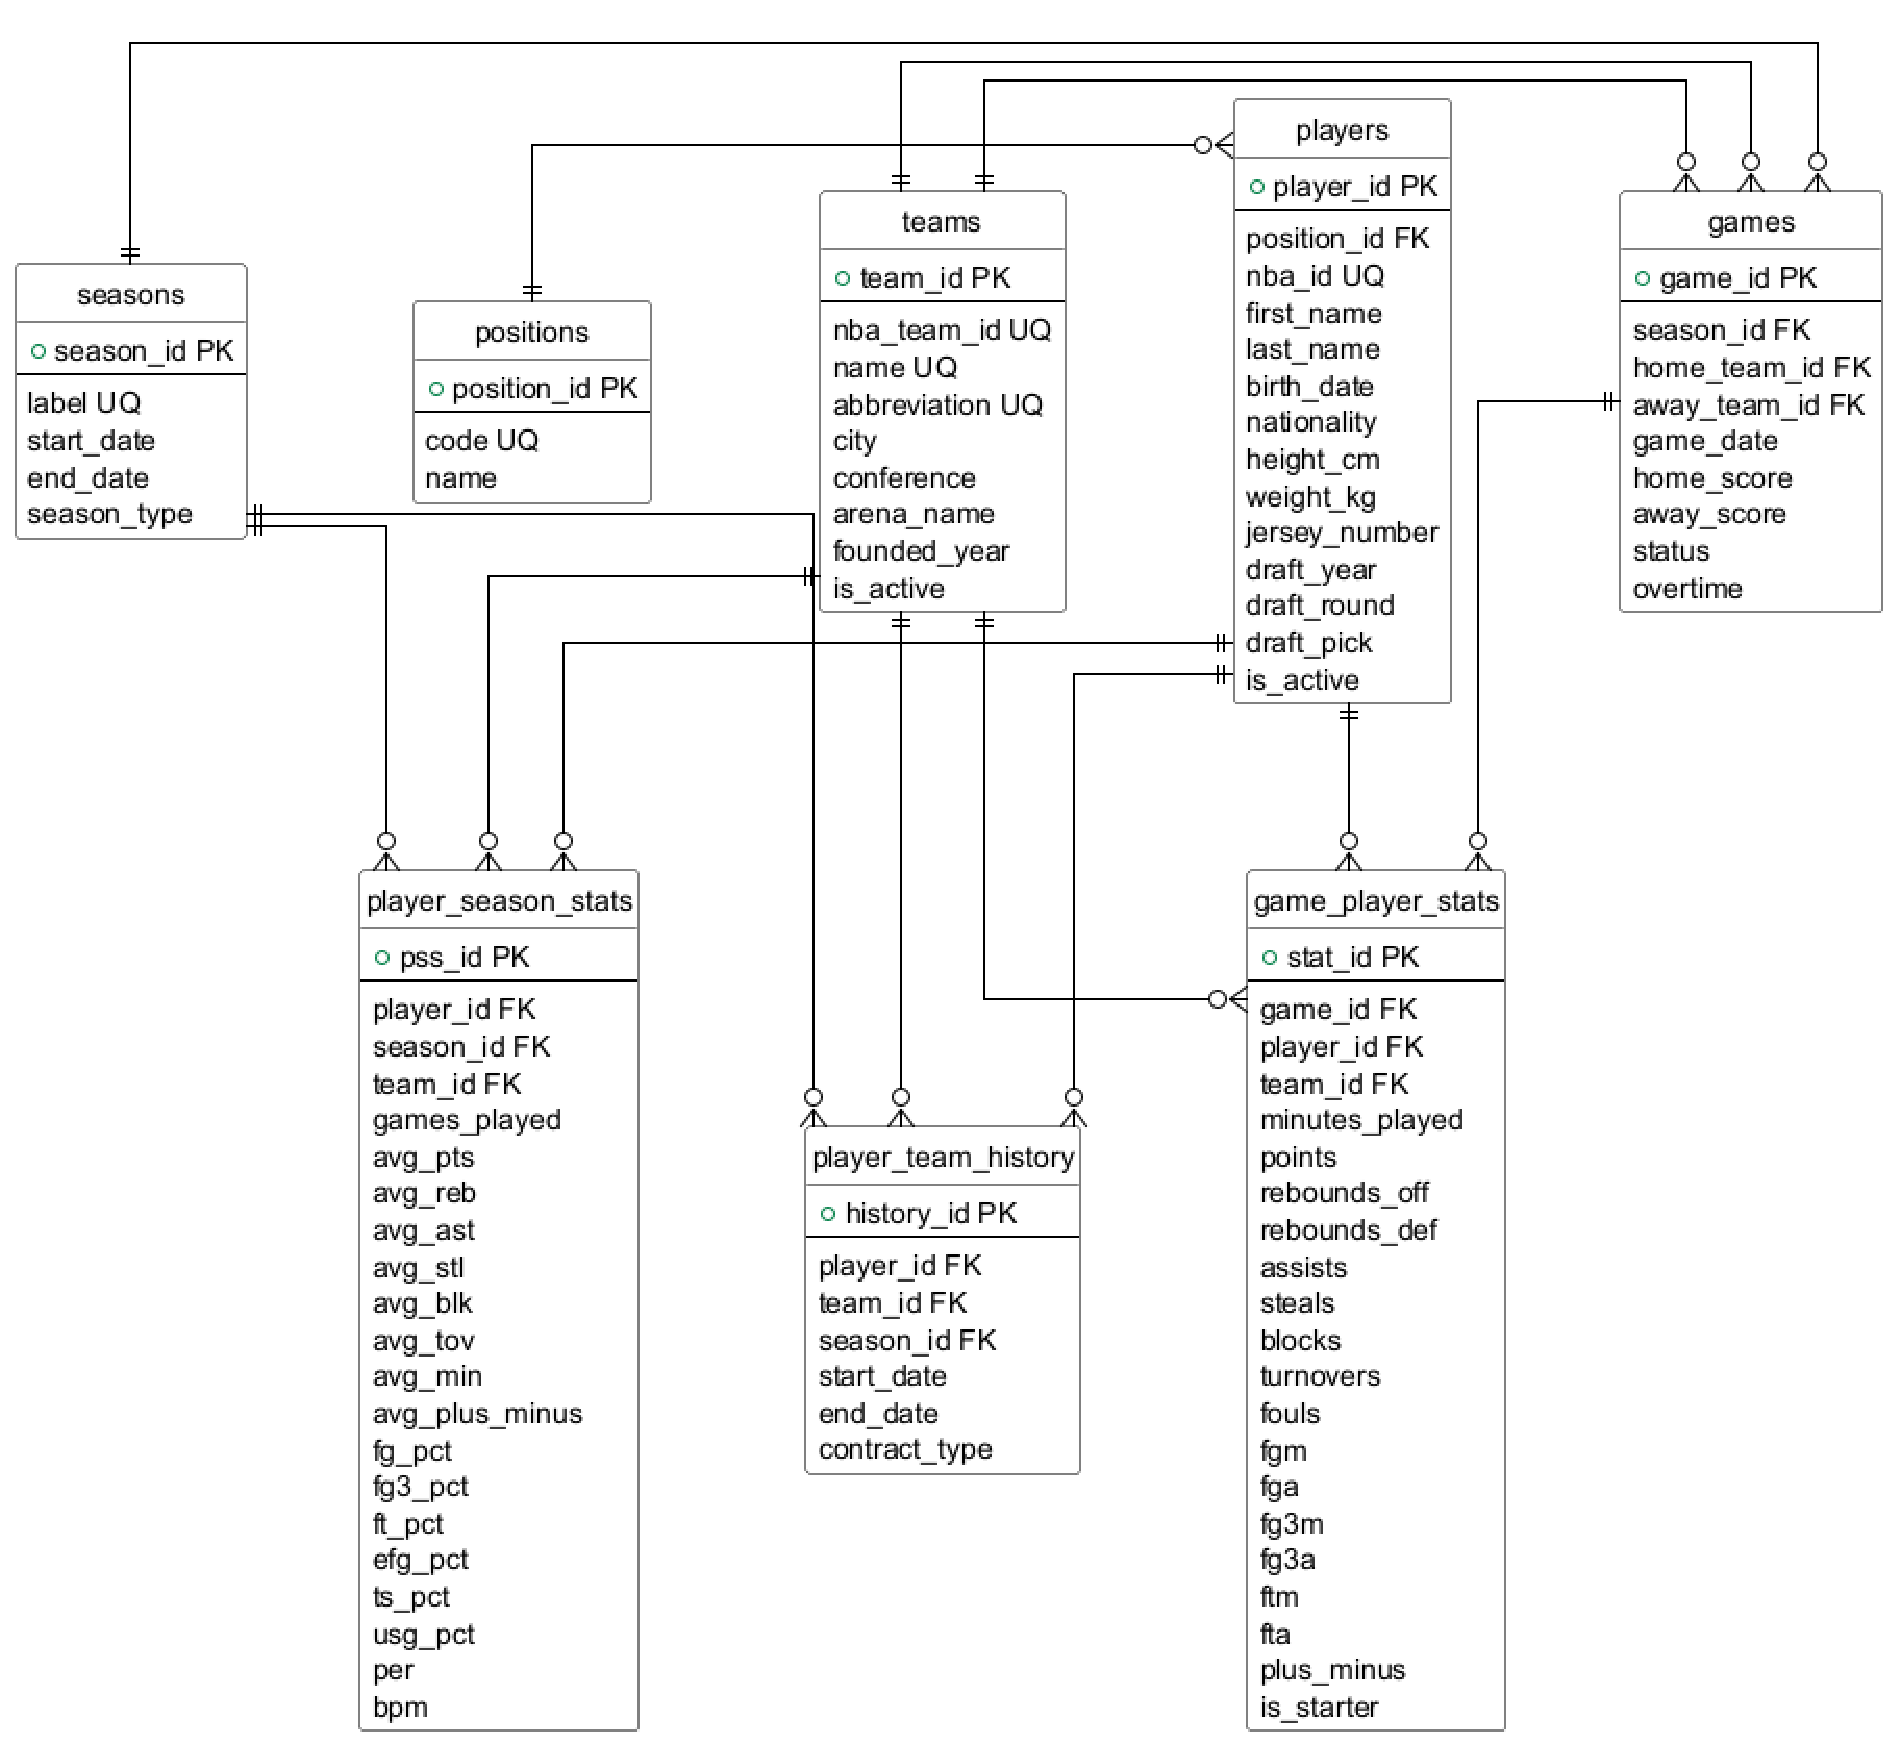
\includegraphics[width=1\textwidth]{../img/relational_schema.pdf}
\caption{Схема реляционной базы данных}
\label{fig:relational-schema}
\end{figure}

{\footnotesize\setlength{\tabcolsep}{4pt}\renewcommand{\arraystretch}{1.12}%

{\normalsize
Для нормализованного хранения игровых позиций спроектирована таблица
\texttt{positions} (табл.~\ref{tab:pos}).
}

\begin{table}[H]
\caption{Справочник игровых позиций}
\label{tab:pos}
\centering
\begin{tabular}{|p{0.22\textwidth}|p{0.28\textwidth}|p{0.42\textwidth}|}
\hline
\textbf{Атрибут} & \textbf{Тип} & \textbf{Ключ / назначение} \\
\hline
position\_id & Целочисленный (автоинкремент) & первичный ключ \\
\hline
code & Строковый фиксированной длины & уникальный; код позиции \\
\hline
name & Строковый & полное название позиции \\
\hline
\end{tabular}
\end{table}

{\normalsize
Интервалы проведения соревнований описываются таблицей
\texttt{seasons} (табл.~\ref{tab:seasons}).
}

\begin{table}[H]
\caption{Справочник сезонов}
\label{tab:seasons}
\centering
\begin{tabular}{|p{0.22\textwidth}|p{0.28\textwidth}|p{0.42\textwidth}|}
\hline
\textbf{Атрибут} & \textbf{Тип} & \textbf{Ключ / назначение} \\
\hline
season\_id & Целочисленный (автоинкремент) & первичный ключ \\
\hline
label & Строковый & уникальный; обозначение сезона, в частности формата 2025-26 \\
\hline
start\_date & Дата & дата начала сезона \\
\hline
end\_date & Дата & дата окончания сезона \\
\hline
season\_type & Строковый & Regular, Playoff, Preseason \\
\hline
\end{tabular}
\end{table}

{\normalsize
Информация о баскетбольных клубах и их домашних аренах хранится в таблице
\texttt{teams} (табл.~\ref{tab:teams}).
}

\begin{table}[H]
\caption{Справочник команд}
\label{tab:teams}
\centering
\begin{tabular}{|p{0.22\textwidth}|p{0.28\textwidth}|p{0.42\textwidth}|}
\hline
\textbf{Атрибут} & \textbf{Тип} & \textbf{Ключ / назначение} \\
\hline
team\_id & Целочисленный (автоинкремент) & первичный ключ \\
\hline
nba\_team\_id & Целочисленный & уникальный; id на NBA.com \\
\hline
name & Строковый & уникальный; полное название \\
\hline
abbreviation & Строковый фиксированной длины & уникальный; аббревиатура \\
\hline
city & Строковый & город базирования \\
\hline
conference & Строковый & допустимые значения: East, West \\
\hline
arena\_name & Строковый & домашняя арена \\
\hline
founded\_year & Целочисленный & год основания \\
\hline
is\_active & Логический & признак активной команды \\
\hline
\end{tabular}
\end{table}

{\normalsize
Для хранения персональных и антропометрических данных баскетболистов
разработана таблица \texttt{players} (табл.~\ref{tab:players}).
}

\begin{table}[H]
\caption{Справочник игроков}
\label{tab:players}
\centering
\begin{tabular}{|p{0.22\textwidth}|p{0.28\textwidth}|p{0.42\textwidth}|}
\hline
\textbf{Атрибут} & \textbf{Тип} & \textbf{Ключ / назначение} \\
\hline
player\_id & Целочисленный (автоинкремент) & первичный ключ \\
\hline
position\_id & Целочисленный & внешний ключ $\rightarrow$ \texttt{positions} \\
\hline
nba\_id & Целочисленный & уникальный; id на NBA.com \\
\hline
first\_name & Строковый & имя \\
\hline
last\_name & Строковый & фамилия \\
\hline
birth\_date & Дата & дата рождения \\
\hline
nationality & Строковый & гражданство \\
\hline
height\_cm & Целочисленный & рост (см) \\
\hline
weight\_kg & Целочисленный & вес (кг) \\
\hline
jersey\_number & Целочисленный & номер на майке (0--99) \\
\hline
draft\_year & Целочисленный & год драфта \\
\hline
draft\_round & Целочисленный & раунд драфта (1 или 2) \\
\hline
draft\_pick & Целочисленный & номер выбора на драфте \\
\hline
is\_active & Логический & действующий игрок \\
\hline
\end{tabular}
\end{table}

{\normalsize
Сведения о проведённых и запланированных матчах фиксируются в таблице
\texttt{games} (табл.~\ref{tab:games}).
}

\begin{table}[H]
\caption{Матчи}
\label{tab:games}
\centering
\begin{tabular}{|p{0.22\textwidth}|p{0.28\textwidth}|p{0.42\textwidth}|}
\hline
\textbf{Атрибут} & \textbf{Тип} & \textbf{Ключ / назначение} \\
\hline
game\_id & Целочисленный (автоинкремент) & первичный ключ \\
\hline
season\_id & Целочисленный & внешний ключ $\rightarrow$ \texttt{seasons} \\
\hline
home\_team\_id & Целочисленный & внешний ключ $\rightarrow$ \texttt{teams}; команда-хозяин \\
\hline
away\_team\_id & Целочисленный & внешний ключ $\rightarrow$ \texttt{teams}; команда-гость \\
\hline
game\_date & Дата & дата матча \\
\hline
home\_score & Целочисленный & счёт хозяев \\
\hline
away\_score & Целочисленный & счёт гостей \\
\hline
status & Строковый & Finished, Scheduled, Postponed \\
\hline
overtime & Целочисленный & число овертаймов (0--6) \\
\hline
\end{tabular}
\end{table}

{\normalsize
Атомарные факты результативности игроков в конкретном матче (основная таблица
фактов) сохраняются в детализированной таблице \texttt{game\_player\_stats}
(табл.~\ref{tab:gps}).
}

\begin{table}[H]
\caption{Факты статистики игрока в матче}
\label{tab:gps}
\centering
\begin{tabular}{|p{0.22\textwidth}|p{0.28\textwidth}|p{0.42\textwidth}|}
\hline
\textbf{Атрибут} & \textbf{Тип} & \textbf{Ключ / назначение} \\
\hline
stat\_id & Целочисленный (автоинкремент) & первичный ключ \\
\hline
game\_id & Целочисленный & внешний ключ $\rightarrow$ \texttt{games}; каскадное удаление \\
\hline
player\_id & Целочисленный & внешний ключ $\rightarrow$ \texttt{players}; запрет удаления при зависимых записях \\
\hline
team\_id & Целочисленный & внешний ключ $\rightarrow$ \texttt{teams}; запрет удаления при зависимых записях \\
\hline
minutes\_played & Вещественный & минуты на площадке \\
\hline
points & Целочисленный & очки (только неотрицательные значения) \\
\hline
rebounds\_off & Целочисленный & подборы в нападении \\
\hline
rebounds\_def & Целочисленный & подборы в защите \\
\hline
assists & Целочисленный & передачи \\
\hline
steals & Целочисленный & перехваты \\
\hline
blocks & Целочисленный & блоки \\
\hline
turnovers & Целочисленный & потери \\
\hline
fouls & Целочисленный & фолы (диапазон 0--6) \\
\hline
fgm, fga & Целочисленный & попадания и попытки с игры \\
\hline
fg3m, fg3a & Целочисленный & попадания и попытки с трёхочковой \\
\hline
ftm, fta & Целочисленный & попадания и попытки штрафных \\
\hline
plus\_minus & Целочисленный & показатель плюс-минус \\
\hline
is\_starter & Логический & признак стартового состава \\
\hline
\multicolumn{3}{|p{\dimexpr\textwidth-2\tabcolsep-2\arrayrulewidth\relax}|}{%
\textbf{Ограничение уникальности:} \texttt{(game\_id, player\_id)}~---
единственность записи игрока в матче} \\
\hline
\end{tabular}
\end{table}

} % end footnotesize (таблицы)

В таблице \texttt{game\_player\_stats} пара полей \texttt{game\_id} и
\texttt{player\_id} закреплена ограничением уникальности. Это исключает
дублирование строк статистики одного игрока в одном матче.

{\footnotesize\setlength{\tabcolsep}{4pt}\renewcommand{\arraystretch}{1.12}%

{\normalsize
Агрегированные статистические показатели и расчётные метрики эффективности за
сезон материализуются в таблице \texttt{player\_season\_stats}
(табл.~\ref{tab:pss}).
}

\begin{table}[H]
\caption{Агрегаты статистики за сезон}
\label{tab:pss}
\centering
\begin{tabular}{|p{0.22\textwidth}|p{0.28\textwidth}|p{0.42\textwidth}|}
\hline
\textbf{Атрибут} & \textbf{Тип} & \textbf{Ключ / назначение} \\
\hline
pss\_id & Целочисленный (автоинкремент) & первичный ключ \\
\hline
player\_id & Целочисленный & внешний ключ $\rightarrow$ \texttt{players}; часть ограничения уникальности \\
\hline
season\_id & Целочисленный & внешний ключ $\rightarrow$ \texttt{seasons}; часть ограничения уникальности \\
\hline
team\_id & Целочисленный & внешний ключ $\rightarrow$ \texttt{teams}; часть ограничения уникальности \\
\hline
games\_played & Целочисленный & число игр в сезоне \\
\hline
avg\_pts & Вещественный & средние очки за матч \\
\hline
avg\_reb & Вещественный & средние подборы за матч \\
\hline
avg\_ast & Вещественный & средние передачи за матч \\
\hline
avg\_stl & Вещественный & средние перехваты за матч \\
\hline
avg\_blk & Вещественный & средние блоки за матч \\
\hline
avg\_tov & Вещественный & средние потери за матч \\
\hline
avg\_min & Вещественный & среднее время на площадке \\
\hline
avg\_plus\_minus & Вещественный & средний плюс-минус \\
\hline
fg\_pct & Вещественный & процент попаданий с игры ($\in [0,1]$) \\
\hline
fg3\_pct & Вещественный & процент трёхочковых ($\in [0,1]$) \\
\hline
ft\_pct & Вещественный & процент штрафных ($\in [0,1]$) \\
\hline
efg\_pct & Вещественный & eFG\% (доля 0--1) \\
\hline
ts\_pct & Вещественный & TS\% (доля 0--1) \\
\hline
usg\_pct & Вещественный & USG\% (доля 0--1) \\
\hline
per & Вещественный & PER \\
\hline
bpm & Вещественный & BPM \\
\hline
\multicolumn{3}{|p{\dimexpr\textwidth-2\tabcolsep-2\arrayrulewidth\relax}|}{%
\textbf{Ограничение уникальности:} \texttt{(player\_id, season\_id, team\_id)}~---
не более одной строки агрегата на игрока, сезон и команду} \\
\hline
\end{tabular}
\end{table}

{\normalsize
Трансферы игроков фиксируются в таблице
\texttt{player\_team\_history} (табл.~\ref{tab:pth}).
}

\begin{table}[H]
\caption{История выступлений игроков}
\label{tab:pth}
\centering
\begin{tabular}{|p{0.22\textwidth}|p{0.28\textwidth}|p{0.42\textwidth}|}
\hline
\textbf{Атрибут} & \textbf{Тип} & \textbf{Ключ / назначение} \\
\hline
history\_id & Целочисленный (автоинкремент) & первичный ключ \\
\hline
player\_id & Целочисленный & внешний ключ $\rightarrow$ \texttt{players}; часть ограничения уникальности \\
\hline
team\_id & Целочисленный & внешний ключ $\rightarrow$ \texttt{teams} \\
\hline
season\_id & Целочисленный & внешний ключ $\rightarrow$ \texttt{seasons} \\
\hline
start\_date & Дата & дата начала выступления \\
\hline
end\_date & Дата & дата окончания (не задана~--- по сей день) \\
\hline
contract\_type & Строковый & Standard, Two-Way, 10-Day и др. \\
\hline
\end{tabular}
\end{table}
} % end footnotesize

\subsection{Соответствие нормальным формам}

Проектирование транзакционной части схемы выполнено с соблюдением требований нормализации до третьей нормальной формы включительно. Это минимизирует избыточность данных и предотвращает аномалии модификации. Для аналитической витрины \newline \texttt{player\_season\_stats} применена контролируемая денормализация с целью оптимизации скорости выполнения запросов~\cite{date}.

\textbf{Первая нормальная форма.} В соответствии с требованиями первой нормальной формы все атрибуты отношений являются атомарными, а скрытые массивы и списки отсутствуют. В схеме нет составных или многозначных атрибутов. Полное имя игрока декомпозировано на скалярные атрибуты имени и фамилии. Рост и вес хранятся как отдельные числовые значения. История трансферов вынесена в отдельную таблицу. Базовые таблицы схемы соответствуют требованиям первой нормальной формы.

\textbf{Вторая нормальная форма.} Отношение находится во второй нормальной форме, если оно соответствует первой нормальной форме и каждый неключевой атрибут функционально полно зависит от любого потенциального ключа. Неключевым является атрибут, не входящий в состав ни одного потенциального ключа.

Потенциальные ключи и неключевые атрибуты спроектированных таблиц приведены в таблице~\ref{tab:potential_keys}.

{\footnotesize\setlength{\tabcolsep}{4pt}\renewcommand{\arraystretch}{1.15}
\begin{table}[H]
\caption{Потенциальные ключи и неключевые атрибуты спроектированных таблиц}
\label{tab:potential_keys}
\centering
\begin{tabular}{|>{\RaggedRight\arraybackslash}p{0.28\textwidth}|>{\RaggedRight\arraybackslash}p{0.26\textwidth}|>{\RaggedRight\arraybackslash}p{0.34\textwidth}|}
\hline
\textbf{Таблица} & \textbf{Потенциальные ключи} & \textbf{Неключевые атрибуты} \\
\hline
\texttt{positions} & \{\texttt{position\_id}\}, \{\texttt{code}\} & \texttt{name} \\
\hline
\texttt{seasons} & \{\texttt{season\_id}\}, \{\texttt{label}\} & \texttt{start\_date}, \texttt{end\_date}, \texttt{season\_type} \\
\hline
\texttt{teams} & \{\texttt{team\_id}\}, \{\texttt{nba\_team\_id}\}, \{\texttt{name}\}, \{\texttt{abbreviation}\} & \texttt{city}, \texttt{conference}, \texttt{arena\_name}, \texttt{founded\_year}, \texttt{is\_active} \\
\hline
\texttt{players} & \{\texttt{player\_id}\}, \{\texttt{nba\_id}\} & \texttt{first\_name}, \texttt{last\_name}, \texttt{birth\_date}, \texttt{nationality}, \texttt{height\_cm}, \texttt{weight\_kg}, \texttt{position\_id}, \texttt{jersey\_number}, \texttt{is\_active}, \texttt{draft\_year}, \texttt{draft\_round}, \texttt{draft\_pick} \\
\hline
\texttt{games} & \{\texttt{game\_id}\} & \texttt{season\_id}, \texttt{home\_team\_id}, \texttt{away\_team\_id}, \texttt{game\_date}, \texttt{home\_score}, \texttt{away\_score}, \texttt{status}, \texttt{overtime} \\
\hline
\texttt{player\_team\_history} & \{\texttt{history\_id}\}, \{\texttt{player\_id}, \texttt{season\_id}, \texttt{team\_id}\} & \texttt{start\_date}, \texttt{end\_date}, \texttt{contract\_type} \\
\hline
\texttt{game\_player\_stats} & \{\texttt{stat\_id}\}, \{\texttt{game\_id}, \texttt{player\_id}\} & \texttt{team\_id}, \texttt{minutes\_played}, \texttt{points}, \texttt{rebounds\_off}, \texttt{rebounds\_def}, \texttt{assists}, \texttt{steals}, \texttt{blocks}, \texttt{turnovers}, \texttt{fouls}, \texttt{fgm}, \texttt{fga}, \texttt{fg3m}, \texttt{fg3a}, \texttt{ftm}, \texttt{fta}, \texttt{plus\_minus}, \texttt{is\_starter} \\
\hline
\end{tabular}
\end{table}}

Для таблиц \texttt{positions}, \texttt{seasons}, \texttt{teams}, \texttt{players} и \texttt{games} все потенциальные ключи состоят из одного атрибута, поэтому частичная зависимость в них невозможна.

Таблицы \texttt{game\_player\_stats} и \texttt{player\_team\_history} имеют составные потенциальные ключи. В \texttt{game\_player\_stats} ключ включает идентификаторы матча и игрока; неключевые атрибуты характеризуют результат конкретного игрока в конкретном матче, и ни один показатель не определяется только идентификатором игрока или только идентификатором матча. Атрибут команды также зависит от обеих частей ключа из-за возможности переходов игрока в течение сезона. В \texttt{player\_team\_history} составной ключ образуют идентификаторы игрока, сезона и команды: одна запись описывает отдельный период выступления, а атрибуты дат начала и окончания и типа контракта зависят от полного ключа, а не от его части. Таким образом, частичные зависимости устранены, и схема соответствует требованиям второй нормальной формы.

\textbf{Третья нормальная форма.} Отношение находится в третьей нормальной форме, если оно соответствует второй нормальной форме и не содержит транзитивных функциональных зависимостей неключевых атрибутов от потенциальных ключей. Это означает отсутствие функциональных зависимостей между самими неключевыми атрибутами.

Анализ неключевых атрибутов базовых таблиц:
\begin{enumerate}
    \item \texttt{positions}: содержит единственный неключевой атрибут названия позиции, что исключает взаимосвязи неключевых атрибутов;
    \item \texttt{seasons}: неключевые атрибуты дат начала и окончания, а также типа сезона не связаны транзитивными зависимостями друг с другом;
    \item \texttt{teams}: неключевые атрибуты города, конференции, названия арены, года основания и активности описывают свойства тридцати уникальных клубов ассоциации и не образуют транзитивных функциональных зависимостей;
    \item \texttt{players}: неключевые атрибуты имени, фамилии, даты рождения, гражданства, физических параметров и драфта не связаны транзитивными зависимостями. Текстовое название позиции вынесено во внешнюю таблицу \texttt{positions}, что исключает транзитивную зависимость через внешний ключ;
    \item \texttt{games}: неключевые атрибуты дат, счета и статуса не связаны транзитивными зависимостями. Названия команд и городов вынесены в таблицу \texttt{teams}, что устраняет транзитивные зависимости через внешние ключи команд;
    \item \texttt{game\_player\_stats}: неключевые атрибуты представляют собой индивидуальные статистические показатели игрока в матче, не связанные транзитивными зависимостями;
    \item \texttt{player\_team\_history}: неключевые атрибуты дат выступления и типа контракта не имеют функциональных зависимостей между собой.
\end{enumerate}

Базовые таблицы схемы соответствуют требованиям третьей нормальной формы.

Аналитическая витрина \texttt{player\_season\_stats} спроектирована как денормализованное отношение. Её потенциальными ключами являются \{\texttt{pss\_id}\} и \{\texttt{player\_id}, \texttt{season\_id}, \texttt{team\_id}\}. Как самостоятельное отношение она удовлетворяет требованиям третьей нормальной формы, поскольку её неключевые атрибуты, представляющие собой средние значения и интегральные метрики, функционально независимы друг от друга. Хранение производных данных в данном случае является контролируемой денормализацией. Данное решение принято с целью повышения производительности аналитических запросов за счет предварительного расчета агрегатов. Это исключает необходимость выполнения ресурсоемких группировок по таблице фактов \texttt{game\_player\_stats} на этапе чтения.
\subsection{Проектирование представлений}

Инкапсуляция базовых таблиц и ограничение прямого доступа спроектированы
через три представления:
\begin{enumerate}
    \item \texttt{v\_player\_rankings}~--- инкапсулирует операцию объединения между
          таблицей агрегатов \texttt{player\_season\_stats} и справочниками
          \texttt{players}, \texttt{teams}. Предоставляет денормализованный
          сводный рейтинг игроков за сезон по базовым и расчётным метрикам,
          скрывая от клиента сложность объединения таблиц;
    \item \texttt{v\_team\_stats}~--- спроектирован для обеспечения функционального требования
          динамического расчёта командной статистики. Выполняет агрегацию
          данных таблицы \newline \texttt{game\_player\_stats} с применением
          статистических функций среднего и суммы в разрезе команды
          и сезона, исключая необходимость хранения избыточной таблицы
          командных фактов;
    \item \texttt{v\_top\_players}~--- обеспечивает безопасность данных для
          публичной роли \texttt{reader}. Является фильтрованным подмножеством
          представления \texttt{v\_player\_rankings} с ограничением выборки
          и сортировкой лидеров по метрике PER.
\end{enumerate}

\subsection{Проектирование индексов}\label{subsec:indexes}

Для обеспечения производительности аналитических запросов (согласно п.~\ref{sec:nfr})
спроектировано создание следующих индексов на базе структуры B-tree~\cite{connolly}:
\begin{enumerate}
    \item \texttt{idx\_gps\_player\_id}~--- индекс по полю \texttt{player\_id}
          в таблице \texttt{game\_player\_stats}; ускоряет выборку всех выступлений
          игрока для агрегации сезонной статистики;
    \item \texttt{idx\_gps\_team\_game}~--- составной индекс по полям
          \texttt{team\_id}, \texttt{game\_id} в таблице \texttt{game\_player\_stats};
          поддерживает агрегацию командной статистики в представлении
          \texttt{v\_team\_stats};
    \item \texttt{idx\_games\_season\_id}~--- индекс по полю \texttt{season\_id}
          в таблице \texttt{games}; ускоряет фильтрацию матчей по сезону;
    \item \texttt{idx\_games\_date}~--- индекс по полю \texttt{game\_date} в таблице
          \texttt{games}; обеспечивает диапазонную фильтрацию по дате проведения
          матча;
    \item \texttt{idx\_pss\_season}~--- индекс по полю \texttt{season\_id} в таблице
          \texttt{player\_season\_stats}; ускоряет выборку рейтингов за конкретный
          сезон;
    \item \texttt{idx\_players\_name}~--- составной индекс по полям
          \texttt{last\_name}, \texttt{first\_name} в таблице \texttt{players};
          поддерживает поиск игрока по фамилии.
\end{enumerate}

Для обеспечения уникальности записей в таблице \texttt{game\_player\_stats}
предусмотрен составной индекс по полям \texttt{(game\_id, player\_id)}, который
дополнительно покрывает запросы поиска по паре «матч~-- игрок». В качестве
алгоритмической основы для всех проектируемых индексов выбрана структура
сбалансированного дерева (B-tree), поскольку она обеспечивает логарифмическую
сложность поиска по предикатам равенства и диапазона.

% Общие параметры блок-схем (ГОСТ 19.701): единая ширина блоков
\newcommand{\flowchartBlockWidth}{6.8cm}
\newcommand{\flowchartBlockHeight}{0.85cm}
\newcommand{\flowchartRightShift}{6.3cm}      % отступ правой колонки (рис. 2.2--2.8)
\newcommand{\flowchartRightShiftSmall}{5.0cm} % компактная схема calculate_ts
\newcommand{\flowchartUpdateVGap}{1.28cm}     % верт. зазор для рис. 2.10
\newcommand{\flowchartUpdateMidExtra}{-0.4cm}   % pro3→pro4, pro4→pro5 (рис. 2.10)
\newcommand{\flowchartTinyVExtra}{-0.15cm}    % микро-добавка (рис. 2.3)
\newcommand{\flowchartDecExpExtra}{-0.45cm}   % dec1 → expected (рис. 2.2)

\tikzset{
  fc base/.style={font=\footnotesize, inner sep=4pt},
  fc arrow/.style={thick,->,>=stealth},
  fc startstop/.style={draw, rectangle, rounded corners=10pt,
    text width=\flowchartBlockWidth, minimum height=\flowchartBlockHeight,
    align=center, fill=white},
  fc process/.style={draw, rectangle,
    text width=\flowchartBlockWidth, minimum height=\flowchartBlockHeight,
    align=center, fill=white},
  fc predefined/.style={draw, rectangle,
    text width=\flowchartBlockWidth, minimum height=\flowchartBlockHeight,
    align=center, fill=white,
    path picture={
      \draw ([xshift=4pt]path picture bounding box.north west) --
            ([xshift=4pt]path picture bounding box.south west);
      \draw ([xshift=-4pt]path picture bounding box.north east) --
            ([xshift=-4pt]path picture bounding box.south east);
    }},
  fc io/.style={draw, trapezium, trapezium left angle=75, trapezium right angle=105,
    trapezium stretches=true,
    text width=\flowchartBlockWidth, minimum height=\flowchartBlockHeight,
    align=center, fill=white},
  fc decision/.style={draw, diamond, aspect=3.2,
    text width=5.0cm, inner sep=1pt,
    minimum height=\flowchartBlockHeight, align=center, fill=white},
}

\newcommand{\flowchartCalculateTs}{%
\begin{figure}[H]
\centering
\begin{tikzpicture}[
    fc base,
    node distance=1.5cm,
    startstop/.style={fc startstop},
    process/.style={fc process},
    io/.style={fc io},
    decision/.style={fc decision},
    arrow/.style={fc arrow}
]
\node (start)  [startstop] {Начало};
\node (pro1)   [process,  below of=start] {$PTS, FGA, FTA := \mathrm{SUM}(\ldots)$};
\node (pro2)   [process,  below of=pro1]
  {$D = 2 \cdot (\mathrm{FGA} + 0{,}44 \cdot \mathrm{FTA})$};
\node (dec1)   [decision, below of=pro2, yshift=-0.5cm] {$D = 0$?};
\node (pro3a)  [io,  right of=dec1, xshift=\flowchartRightShiftSmall] {Вывод:\\ значение не определено};
\node (pro3b)  [io,  below of=dec1, yshift=-0.5cm]
  {Возврат $\mathrm{PTS} / D$};
\node (stop)   [startstop, below of=pro3b] {Конец};

\draw [arrow] (start)  -- (pro1);
\draw [arrow] (pro1)   -- (pro2);
\draw [arrow] (pro2)   -- (dec1);
\draw [arrow] (dec1)   -- node[anchor=south] {Да}  (pro3a);
\draw [arrow] (dec1)   -- node[anchor=east]  {Нет} (pro3b);
\draw [arrow] (pro3b)  -- (stop);
\draw [arrow] (pro3a)  |- (stop);
\end{tikzpicture}
\caption{Схема алгоритма вычисления функции \texttt{calculate\_ts}}
\label{fig:algo-ts}
\end{figure}
}

\newcommand{\flowchartCalculateEfg}{%
\begin{figure}[H]
\centering
\begin{tikzpicture}[
    fc base,
    node distance=1.8cm,
    startstop/.style={fc startstop},
    process/.style={fc process},
    io/.style={fc io},
    decision/.style={fc decision},
    arrow/.style={fc arrow}
]
\node (start)  [startstop] {Начало};
\node (agg)    [process,  below of=start]
  {$FGM, FG3M, FGA := \mathrm{SUM}(\ldots)$ \\ из \texttt{game\_player\_stats}};
\node (dec1)   [decision, below of=agg] {$\mathrm{FGA} = 0$?};
\node (null1)  [io,  right of=dec1, xshift=\flowchartRightShift] {Вывод:\\ значение не определено};
\node (ret)    [io,  below of=dec1]
  {Возврат $\displaystyle\frac{\mathrm{FGM}+0{,}5\cdot\mathrm{FG3M}}{\mathrm{FGA}}$};
\node (stop)   [startstop, below of=ret] {Конец};

\draw [arrow] (start) -- (agg);
\draw [arrow] (agg)   -- (dec1);
\draw [arrow] (dec1)  -- node[above] {Да} (null1);
\draw [arrow] (dec1)  -- node[right] {Нет} (ret);
\draw [arrow] (ret)   -- (stop);
\draw [arrow] (null1.east) -- ++(0.6,0) |- (stop);
\end{tikzpicture}
\caption{Схема алгоритма вычисления функции \texttt{calculate\_efg}}
\label{fig:algo-efg}
\end{figure}
}

\newcommand{\flowchartCalculateUsg}{%
\begin{figure}[H]
\centering
\begin{tikzpicture}[
    fc base,
    node distance=1.8cm,
    startstop/.style={fc startstop},
    process/.style={fc process},
    io/.style={fc io},
    decision/.style={fc decision},
    arrow/.style={fc arrow}
]
\node (start)  [startstop] {Начало};
\node (tid)    [process,  below of=start]
  {Определить team\_id \\ (параметр или последняя игра)};
\node (dec0)   [decision, below of=tid, yshift=-0.2cm] {team\_id IS NULL?};
\node (null0)  [io,  right of=dec0, xshift=\flowchartRightShift] {Вывод:\\ значение не определено};
\node (aggP)   [process,  below of=dec0, yshift=-0.2cm]
  {$pFGA, pFTA, pTOV, pMP :=$ \\ $\mathrm{SUM}(\ldots)$ игрока};
\node (dec1)   [decision, below of=aggP, yshift=-0.2cm] {$pMP < 1$?};
\node (null1)  [io,  right of=dec1, xshift=\flowchartRightShift] {Вывод:\\ значение не определено};
\node (aggT)   [process,  below of=dec1, yshift=-0.2cm]
  {$tmFGA, tmFTA, tmTOV, tmMP :=$ \\ $\mathrm{SUM}(\ldots)$ команды};
\node (denom)  [process,  below of=aggT, yshift=-0.2cm]
  {$denom := pMP \cdot (tmFGA + 0{,}44 \cdot tmFTA + tmTOV)$};
\node (dec2)   [decision, below of=denom, yshift=-0.2cm] {denom $= 0$?};
\node (null2)  [io,  right of=dec2, xshift=\flowchartRightShift] {Вывод:\\ значение не определено};
\node (ret)    [io,  below of=dec2, yshift=-0.2cm]
  {Возврат $\displaystyle\frac{(pFGA+0{,}44\cdot pFTA+pTOV)\cdot\frac{tmMP}{5}}{denom}$};
\node (stop)   [startstop, below of=ret] {Конец};

\draw [arrow] (start) -- (tid);
\draw [arrow] (tid)   -- (dec0);
\draw [arrow] (dec0)  -- node[above] {Да} (null0);
\draw [arrow] (dec0)  -- node[right] {Нет} (aggP);
\draw [arrow] (aggP)  -- (dec1);
\draw [arrow] (dec1)  -- node[above] {Да} (null1);
\draw [arrow] (dec1)  -- node[right] {Нет} (aggT);
\draw [arrow] (aggT)  -- (denom);
\draw [arrow] (denom) -- (dec2);
\draw [arrow] (dec2)  -- node[above] {Да} (null2);
\draw [arrow] (dec2)  -- node[right] {Нет} (ret);
\draw [arrow] (ret)   -- (stop);

\draw [arrow] (null0.east) -- ++(0.5,0) coordinate (bus) |- (stop);
\draw [arrow] (null1.east) -- (null1.east -| bus);
\draw [arrow] (null2.east) -- (null2.east -| bus);
\end{tikzpicture}
\caption{Схема алгоритма вычисления функции \texttt{calculate\_usg}}
\label{fig:algo-usg}
\end{figure}
}

\newcommand{\flowchartCalculatePer}{%
\begin{figure}[H]
\centering
\begin{tikzpicture}[
    fc base,
    node distance=1.8cm,
    startstop/.style={fc startstop},
    process/.style={fc process},
    predefined/.style={fc predefined},
    io/.style={fc io},
    decision/.style={fc decision},
    arrow/.style={fc arrow}
]
\node (start) [startstop] {Начало};
\node (agg)   [process,  below of=start]
  {$PTS, TRB, AST, STL, BLK,$ \\ $TOV, PF, FGM/FGA, FTM/FTA, MP := \mathrm{SUM}(\ldots)$};
\node (dec1)  [decision, below of=agg] {$\mathrm{MP} < 50$?};
\node (null1) [io,  right of=dec1, xshift=\flowchartRightShift] {Вывод:\\ значение не определено};
\node (uper)  [process,  below of=dec1]
  {$\mathrm{uPER} = (\mathrm{PTS}+\mathrm{TRB}+\ldots - \mathrm{TOV}-\mathrm{PF}-\Delta\mathrm{FG}-0{,}44\cdot\Delta\mathrm{FT}) \cdot \tfrac{48}{\mathrm{MP}}$};
\node (lg)    [predefined,  below of=uper]
  {Вычисление lg\_aPER: \\ AVG(uPER) по игрокам с MP $> 100$};
\node (dec2)  [decision, below of=lg] {lg\_aPER $= 0$ или NULL?};
\node (fix)   [process,  right of=dec2, xshift=\flowchartRightShift] {lg\_aPER $= 15{,}0$};
\node (ret)   [io,  below of=dec2]
  {Возврат $\mathrm{uPER} \cdot 15\,/\,\mathrm{lg\_aPER}$};
\node (stop)  [startstop, below of=ret] {Конец};

\draw [arrow] (start) -- (agg);
\draw [arrow] (agg)   -- (dec1);
\draw [arrow] (dec1)  -- node[above] {Да} (null1);
\draw [arrow] (dec1)  -- node[right] {Нет} (uper);
\draw [arrow] (uper)  -- (lg);
\draw [arrow] (lg)    -- (dec2);
\draw [arrow] (dec2)  -- node[above] {Да} (fix);
\draw [arrow] (dec2)  -- node[right] {Нет} (ret);
\draw [arrow] (fix)   |- (ret);
\draw [arrow] (ret)   -- (stop);
\draw [arrow] (null1.east) -- ++(1.0,0) |- (stop);
\end{tikzpicture}
\caption{Схема алгоритма вычисления функции \texttt{calculate\_per}}
\label{fig:algo-per}
\end{figure}
}

\newcommand{\flowchartCalculateBpm}{%
\begin{figure}[H]
\centering
\begin{tikzpicture}[
    fc base,
    node distance=1.8cm,
    startstop/.style={fc startstop},
    process/.style={fc process},
    predefined/.style={fc predefined},
    io/.style={fc io},
    decision/.style={fc decision},
    arrow/.style={fc arrow}
]
\node (start) [startstop] {Начало};
\node (agg)   [process,  below of=start]
  {$PTS, TRB, AST, STL,$ \\ $BLK, TOV, PF, MP := \mathrm{SUM}(\ldots)$};
\node (dec1)  [decision, below of=agg] {$\mathrm{MP} < 50$?};
\node (null1) [io,  right of=dec1, xshift=\flowchartRightShift] {Вывод:\\ значение не определено};
\node (norm)  [process,  below of=dec1]
  {Нормировка на 100 мин: $X_{100} = X \cdot 100\,/\,\mathrm{MP}$};
\node (raw)   [process,  below of=norm]
  {raw $= 0{,}123\cdot\mathrm{PTS}_{100}+0{,}234\cdot\mathrm{TRB}_{100}+0{,}689\cdot\mathrm{AST}_{100}$ \\ $+\,0{,}445\cdot\mathrm{STL}_{100}+0{,}407\cdot\mathrm{BLK}_{100}-0{,}605\cdot\mathrm{TOV}_{100}-0{,}086\cdot\mathrm{PF}_{100}$};
\node (lg)    [predefined,  below of=raw]
  {Вычисление lg\_avg: \\ AVG(raw) по игрокам с MP $> 100$};
\node (ret)   [io,  below of=lg] {Возврат raw $-$ lg\_avg};
\node (stop)  [startstop, below of=ret] {Конец};

\draw [arrow] (start) -- (agg);
\draw [arrow] (agg)   -- (dec1);
\draw [arrow] (dec1)  -- node[above] {Да} (null1);
\draw [arrow] (dec1)  -- node[right] {Нет} (norm);
\draw [arrow] (norm)  -- (raw);
\draw [arrow] (raw)   -- (lg);
\draw [arrow] (lg)    -- (ret);
\draw [arrow] (ret)   -- (stop);
\draw [arrow] (null1.east) -- ++(0.6,0) |- (stop);
\end{tikzpicture}
\caption{Схема алгоритма вычисления функции \texttt{calculate\_bpm}}
\label{fig:algo-bpm}
\end{figure}
}

\newcommand{\flowchartTriggerScore}{%
\begin{figure}[H]
\centering
\begin{tikzpicture}[
    fc base,
    node distance=1.8cm,
    startstop/.style={fc startstop},
    process/.style={fc process},
    predefined/.style={fc predefined},
    io/.style={fc io},
    decision/.style={fc decision},
    arrow/.style={fc arrow}
]
\node (start) [startstop] {Начало};
\node (get)   [io,  below of=start]
  {Получить status, home/away\_id, \\ счёт из \texttt{games} по game\_id};
\node (dec1)  [decision, below of=get] {status $\neq$ 'Finished' \\ или счёт NULL?};
\node (skip)  [io,  right of=dec1, xshift=\flowchartRightShift] {Возврат NEW/OLD};
\node (exp)   [process,  below of=dec1, yshift=\flowchartDecExpExtra]
  {$expected :=$ счёт команды \\ (\texttt{home\_score} или \texttt{away\_score})};
\node (loop)  [predefined,  below of=exp]
  {Для каждой команды в матче: \\ $teamPoints := \mathrm{SUM(points)}$};
\node (dec2)  [decision, below of=loop] {$teamPoints \neq expected$?};
\node (exc)   [io,  right of=dec2, xshift=\flowchartRightShift] {RAISE EXCEPTION};
\node (ret)   [io,  below of=dec2] {Возврат NEW/OLD};
\node (stop)  [startstop, below of=ret] {Конец};

\draw [arrow] (start) -- (get);
\draw [arrow] (get)   -- (dec1);
\draw [arrow] (dec1)  -- node[above] {Да} (skip);
\draw [arrow] (dec1)  -- node[right] {Нет} (exp);
\draw [arrow] (exp)   -- (loop);
\draw [arrow] (loop)  -- (dec2);
\draw [arrow] (dec2)  -- node[above] {Да} (exc);
\draw [arrow] (dec2)  -- node[right] {Нет} (ret);
\draw [arrow] (ret)   -- (stop);

\draw [arrow] (skip.east) -- ++(0.6,0) coordinate (bus) |- (stop);
\draw [arrow] (exc.east) -- (exc.east -| bus);
\end{tikzpicture}
\caption{Схема алгоритма функции-триггера \texttt{trg\_validate\_team\_score\_row}}
\label{fig:algo-trg-score}
\end{figure}
}

\newcommand{\flowchartTriggerSeasonStats}{%
\begin{figure}[H]
\centering
\begin{tikzpicture}[
    fc base,
    node distance=1.8cm,
    startstop/.style={fc startstop},
    process/.style={fc process},
    predefined/.style={fc predefined},
    io/.style={fc io},
    decision/.style={fc decision},
    arrow/.style={fc arrow}
]
\node (start) [startstop] {Начало};
\node (get)   [io,  below of=start]
  {Получить список уникальных season\_id \\ из новых строк};
\node (dec1)  [decision, below of=get] {Список season\_id пуст?};
\node (null1) [io,  right of=dec1, xshift=\flowchartRightShift] {Вывод:\\ значение не определено};
\node (call)  [predefined,  below of=dec1, yshift=\flowchartTinyVExtra]
  {Для каждого season\_id: \\ \texttt{CALL update\_season\_stats(season\_id)}};
\node (ret)   [io,  below of=call, yshift=\flowchartTinyVExtra] {Вывод:\\ значение не определено};
\node (stop)  [startstop, below of=ret] {Конец};

\draw [arrow] (start) -- (get);
\draw [arrow] (get)   -- (dec1);
\draw [arrow] (dec1)  -- node[above] {Да} (null1);
\draw [arrow] (dec1)  -- node[right] {Нет} (call);
\draw [arrow] (call)  -- (ret);
\draw [arrow] (ret)   -- (stop);
\draw [arrow] (null1.east) -- ++(0.6,0) |- (stop);
\end{tikzpicture}
\caption{Схема алгоритма функции-триггера \texttt{trg\_update\_season\_stats\_func}}
\label{fig:algo-trg-update}
\end{figure}
}

\newcommand{\flowchartTeamStats}{%
\begin{figure}[H]
\centering
\begin{tikzpicture}[
    fc base,
    node distance=1.2cm,
    startstop/.style={fc startstop},
    process/.style={fc process},
    arrow/.style={fc arrow}
]
\node (start) [startstop] {Начало построения представления \texttt{v\_team\_stats}};
\node (join)  [process, below of=start]
  {Соединение \texttt{game\_player\_stats} с \texttt{games}};
\node (role)  [process, below of=join]
  {Определение команды по \texttt{home\_team\_id} и \texttt{away\_team\_id}};
\node (group) [process, below of=role]
  {Группировка по \texttt{team\_id} и \texttt{season\_id}};
\node (agg)   [process, below of=group]
  {teamTotals := SUM(очки, подборы, \\ передачи, потери, броски)};
\node (avg)   [process, below of=agg]
  {Деление накопленных сумм на число матчей команды};
\node (stop)  [startstop, below of=avg] {Вывод средних командных показателей};

\draw [arrow] (start) -- (join);
\draw [arrow] (join)  -- (role);
\draw [arrow] (role)  -- (group);
\draw [arrow] (group) -- (agg);
\draw [arrow] (agg)   -- (avg);
\draw [arrow] (avg)   -- (stop);
\end{tikzpicture}
\caption{Схема алгоритма агрегирования командной статистики в представлении \texttt{v\_team\_stats}}
\label{fig:algo-team-stats}
\end{figure}
}

\newcommand{\flowchartUpdateSeasonStats}{%
\begin{figure}[H]
\centering
\begin{tikzpicture}[
    fc base,
    node distance=\flowchartUpdateVGap,
    startstop/.style={fc startstop},
    process/.style={fc process},
    predefined/.style={fc predefined},
    arrow/.style={fc arrow}
]
\node (start) [startstop] {Начало транзакции};
\node (pro1)  [process, below of=start]
  {Группировка по \texttt{player\_id}, \texttt{team\_id}: базовые агрегаты};
\node (pro2)  [predefined, below of=pro1]
  {Подзапрос TmFGA/TmFTA/TmTOV по (\texttt{game\_id}, \texttt{team\_id}) для USG};
\node (pro3)  [process, below of=pro2]
  {Двухпроходный расчёт лигового среднего (PER, BPM)};
\node (pro4)  [predefined, below of=pro3, yshift=\flowchartUpdateMidExtra]
  {Вызов \texttt{calculate\_efg}, \texttt{calculate\_ts}, \\ \texttt{calculate\_usg}, \texttt{calculate\_per}, \texttt{calculate\_bpm}};
\node (pro5)  [process, below of=pro4, yshift=\flowchartUpdateMidExtra]
  {Вставка с обновлением в таблицу \texttt{player\_season\_stats}};
\node (stop)  [startstop, below of=pro5] {Конец транзакции};

\draw [arrow] (start) -- (pro1);
\draw [arrow] (pro1)  -- (pro2);
\draw [arrow] (pro2)  -- (pro3);
\draw [arrow] (pro3)  -- (pro4);
\draw [arrow] (pro4)  -- (pro5);
\draw [arrow] (pro5)  -- (stop);
\end{tikzpicture}
\caption{Схема алгоритма хранимой процедуры \texttt{update\_season\_stats}}
\label{fig:algo-update}
\end{figure}
}


\section{Проектирование ограничений целостности}\label{sec:integrity-design}

Помимо ограничений первичных и внешних ключей, на уровне базы данных
спроектирована логика защиты бизнес-правил.

Удаление матча вызывает каскадное удаление связанной статистики.
Для справочников игроков и команд физическое удаление на уровне внешних ключей
запрещено; применяется логическое удаление флагом активности.

\textbf{Ограничения-проверки (предикатные).}
Обеспечивают согласованность бросков: \newline \texttt{fg3m}~$\le$~\texttt{fgm},
\texttt{fgm}~$\le$~\texttt{fga}; диапазон фолов от~0 до~6.
Для таблицы \texttt{games} задано ограничение, запрещающее совпадение
команды-хозяина и команды-гостя (\texttt{home\_team\_id} $\neq$
\texttt{away\_team\_id}). Для \texttt{player\_team\_history}~--- ограничение,
требующее, чтобы дата начала не превышала дату окончания
(\texttt{start\_date} $\le$ \texttt{end\_date}).

\textbf{Процедурные ограничения целостности (триггеры).}
На таблице \texttt{game\_player\_stats} предусмотрены два триггера.
Функция-триггер \texttt{trg\_validate\_team\_score\_row} проверяет
бизнес-правило предметной области: сумма очков всех игроков команды
в завершённом матче должна совпадать с итоговым командным счётом.
Проверка выполняется только для матчей со статусом \texttt{Finished}
и заполненным счётом~--- незавершённые матчи пропускаются без проверки.
Для каждой команды, присутствующей в таблице фактов данного матча,
вычисляется сумма очков и сравнивается с \texttt{home\_score}
или \texttt{away\_score}. При несовпадении триггер поднимает исключение
и инициирует откат транзакции в её конце.
Поскольку протокол матча загружается пакетно, проверка суммы очков
должна выполняться не после каждой отдельной строки, а по завершении
всей транзакции~--- после загрузки статистики всех игроков команды.
Ограничение по счёту применимо к полностью обработанным данным:
игроки, не принявшие участие в матче, в таблицу фактов
\texttt{game\_player\_stats} не вносятся; загружаемые источники должны
обеспечивать атрибуцию всех очков конкретным игрокам.
Схема алгоритма функции-триггера приведена на рисунке~\ref{fig:algo-trg-score}.
\flowchartTriggerScore

Триггеры \texttt{trg\_update\_season\_stats\_func} и
\texttt{trigger\_update\_season\_stats} обеспечивают автоматическое
обновление витрины \texttt{player\_season\_stats} после каждой пакетной
вставки в таблицу фактов. С помощью механизма переходных таблиц триггер
извлекает список уникальных \texttt{season\_id} из всего пакета вставленных
строк. Затем в цикле вызывается процедура \texttt{update\_season\_stats}
для каждого затронутого сезона. Это гарантирует корректный пересчёт витрины
даже при массовой загрузке исторических данных, затрагивающих несколько
разных турниров одновременно. Триггер срабатывает на уровне оператора,
что исключает многократный пересчёт витрины при пакетной загрузке данных.
Схема алгоритма функции-триггера приведена на рисунке~\ref{fig:algo-trg-update}.
\flowchartTriggerSeasonStats

\section{Проектирование алгоритмов обработки данных}\label{sec:algorithms-design}

\subsection{Алгоритмы расчёта метрик игроков}\label{subsec:metric-algorithms}

Расчёт метрик делегирован СУБД. Обработка нулевых знаменателей через
возврат неопределённого значения исключает неквалифицированных игроков
из агрегаций.

Функция \texttt{calculate\_ts} рассчитывает истинный процент бросков
(формула~(1.2)) на основе сезонных агрегатов из \texttt{game\_player\_stats}.
При нулевом знаменателе возвращается неопределённое значение.
Схема алгоритма вычисления приведена на рисунке~\ref{fig:algo-ts}.
\flowchartCalculateTs

Функция \texttt{calculate\_efg} рассчитывает эффективный процент бросков
(формула~(1.1)) на основе сезонных агрегатов. Отсутствие попыток броска
обрабатывается возвратом неопределённого значения для предотвращения
деления на ноль.
Схема алгоритма вычисления приведена на рисунке~\ref{fig:algo-efg}.
\flowchartCalculateEfg

Функция \texttt{calculate\_usg} вычисляет долю командных владений,
завершаемых игроком, по формуле~(1.3). Алгоритм требует двух проходов:
суммирования индивидуальных показателей игрока и вычисления командных
агрегатов по общим матчам. Функция возвращает неопределённое значение в трёх случаях: команда игрока не
определена, суммарное время на площадке менее одной минуты, либо командный
знаменатель равен нулю.
Схема алгоритма вычисления приведена на рисунке~\ref{fig:algo-usg}.
\flowchartCalculateUsg

Функция \texttt{calculate\_per} вычисляет рейтинг эффективности игрока
по упрощённой методологии Холлинджера (формулы~1.4--1.6). Алгоритм
двухпроходный. На первом проходе вычисляется ненормализованный вклад игрока
uPER на основе сезонных сумм всех базовых показателей, нормированных на
48~минут. Игроки с суммарным временем менее 50~минут за сезон исключаются
из расчёта. На втором проходе вычисляется среднее значение по лиге.
При неопределённом лиговом среднем значение принудительно устанавливается
в базовый ориентир 15,0.
Схема алгоритма вычисления приведена на рисунке~\ref{fig:algo-per}.
\flowchartCalculatePer

Функция \texttt{calculate\_bpm} вычисляет вклад игрока относительно
среднего по лиге по упрощённой линейной аппроксимации BPM
(формулы~1.7--1.8). Все показатели нормируются на 100~минут игрового
времени, после чего взвешиваются фиксированными коэффициентами модели
Майерса. Игроки с менее чем 50~минутами дисквалифицируются. Лиговое среднее
вычитается из сырого значения, поэтому среднее BPM по лиге после нормировки
равно нулю.
Схема алгоритма вычисления приведена на рисунке~\ref{fig:algo-bpm}.
\flowchartCalculateBpm

\subsection{Алгоритм агрегирования командной статистики}

Командная статистика вычисляется динамически через представление
\texttt{v\_team\_stats}, исключая дублирование данных в отдельной таблице.
Для каждой пары «команда~-- сезон» представление объединяет строки
\texttt{game\_player\_stats} с таблицей \texttt{games} (только завершённые матчи),
группирует статистику игроков по \texttt{(team\_id, season\_id, game\_id)},
суммирует показатели внутри каждого матча и усредняет результат по числу матчей.
Показатели \texttt{efg\_pct} и \texttt{ts\_pct} вычисляются по сезонным суммам
бросков. Результирующий набор содержит средние очки, подборы, передачи, потери
и эффективные показатели команды за матч.
Схема алгоритма агрегирования приведена на рисунке~\ref{fig:algo-team-stats}.
\flowchartTeamStats

\subsection{Алгоритм массового обновления агрегатов}\label{subsec:bulk-update}

Процедура \texttt{update\_season\_stats} пересчитывает витрину
\texttt{player\_season\_stats} для указанного сезона. Алгоритм спроектирован
с отказом от курсоров: применяется одна множественная вставка по результатам
выборки с последующим обновлением при конфликте (вставка с обновлением).
Логика процедуры включает
пять шагов:
\begin{enumerate}
    \item агрегация по \texttt{(player\_id, team\_id)} из \texttt{game\_player\_stats}
          за сезон: средние показатели, проценты бросков, отбор строк с
          $\sum \mathrm{MP} \geq 50$;
    \item для каждой квалифицированной строки вызов \texttt{calculate\_usg}, внутри
          которого командные $\mathrm{TmFGA}$, $\mathrm{TmFTA}$, $\mathrm{TmTOV}$
          и $\mathrm{TmMP}$ суммируются по всем игрокам команды в матчах, где
          участвовал данный игрок (фильтр по \texttt{game\_id} и \texttt{team\_id});
    \item для \texttt{calculate\_per} и \texttt{calculate\_bpm}~--- двухпроходный
          расчёт: сначала вычисляется ненормализованный показатель игрока, затем
          среднее по лиге за сезон (только игроки с $\sum \mathrm{MP} > 100$),
          после чего результат нормируется относительно лигового среднего;
    \item вызов \texttt{calculate\_efg} и \texttt{calculate\_ts} по сезонным
          суммам игрока;
    \item вставка с обновлением в \texttt{player\_season\_stats} по ключу
          \texttt{(player\_id, season\_id, team\_id)}.
\end{enumerate}

Схема алгоритма хранимой процедуры приведена на рисунке~\ref{fig:algo-update}.
\flowchartUpdateSeasonStats

\section{Проектирование ролевой модели доступа}\label{sec:roles}

В базе данных определены три роли: \texttt{db\_admin}, \texttt{analyst} и
\texttt{reader}. Администратору выданы полные права на таблицы,
последовательности и функции схемы. Аналитику доступны выборка из таблиц и
выполнение расчётных функций. Читатель работает исключительно через
представления без прямого доступа к базовым таблицам. Создание и изменение
структуры объектов базы данных выполняются от имени выделенного
пользователя-владельца схемы при развёртывании. Ограничение доступа роли
\texttt{reader} к полному представлению \texttt{v\_player\_rankings} и выдача прав
только на \texttt{v\_top\_players} обусловлены бизнес-логикой: публичным пользователям
доступна лишь краткая сводка лидеров, в то время как полные аналитические выгрузки
предназначены только для аналитиков.
Матрица прав доступа к объектам базы данных приведена в таблице~\ref{tab:acl-matrix}.

\begin{table}[H]
\caption{Матрица прав доступа к объектам базы данных}
\label{tab:acl-matrix}
\centering
\begin{tabular}{|p{0.46\textwidth}|p{0.12\textwidth}|p{0.12\textwidth}|p{0.12\textwidth}|}
\hline
\textbf{Объект} & \textbf{db\_admin} & \textbf{analyst} & \textbf{reader} \\
\hline
positions, seasons, teams, players & полный доступ & чтение & --- \\
\hline
games, game\_player\_stats & полный доступ & чтение & --- \\
\hline
player\_season\_stats, player\_team\_history & полный доступ & чтение & --- \\
\hline
Функции calculate\_* & выполнение & выполнение & --- \\
\hline
v\_team\_stats, v\_top\_players & --- & чтение & чтение \\
\hline
v\_player\_rankings & чтение & чтение & --- \\
\hline
\end{tabular}
\end{table}

\section{Проектирование программного обеспечения и кэширования}

\subsection{Архитектура приложения}\label{subsec:app-architecture}

Программный комплекс построен по трёхзвенной архитектуре. Уровень представления
формирует HTTP-запросы к серверу. Уровень приложения~--- REST
API-сервер, выполняющий маршрутизацию запросов, проверку авторизации и вызов
процедур СУБД. Уровень данных~--- реляционная СУБД и in-memory кэш,
взаимодействие которых описано в подразделе~\ref{subsec:cache}.

API организован в пять групп маршрутов (\texttt{players}, \texttt{teams},
\texttt{stats}, \texttt{league}, \texttt{admin}), соответствующих вариантам
использования из раздела~\ref{sec:use-cases}. Итого спроектировано 22~бизнес-маршрута.

Компонентная диаграмма трёхзвенной архитектуры приведена на
рисунке~\ref{fig:arch-components}. Уровень представления спроектирован
в виде одностраничного веб-приложения (SPA); уровень приложения~---
асинхронный REST API сервер; уровень данных~--- реляционная СУБД,
дополненная in-memory хранилищем формата «ключ-значение».

\begin{figure}[H]
\centering
\begin{tikzpicture}[
    scale=0.95, transform shape,
    every node/.style={font=\small},
    layer/.style={draw, thick, rounded corners=6pt,
      minimum width=3.4cm, minimum height=1.2cm,
      align=center},
    store/.style={draw, thick, cylinder, shape border rotate=90,
      minimum width=2.8cm, minimum height=1.2cm, aspect=0.2,
      align=center},
    arrow/.style={thick,->,>=stealth},
    label/.style={font=\footnotesize, midway}
]

\node (react) [layer, fill=white] at (0, 0)
  {\textbf{Веб-клиент (SPA)}};

\node (api) [layer, fill=white] at (6, 0)
  {\textbf{REST API сервер}};

\node (pg) [store, fill=white] at (12.5, 1.5)
  {\textbf{Реляционная СУБД}};

\node (redis) [store, fill=white] at (12.5, -1.5)
  {\textbf{In-memory хранилище}};

% Arrows React <-> API
\draw [arrow] ([yshift=5pt]react.east) -- node[label, above] {HTTP / REST} ([yshift=5pt]api.west);
\draw [arrow, dashed] ([yshift=-5pt]api.west) -- node[label, below] {JSON} ([yshift=-5pt]react.east);

% Arrows API <-> DB
\draw [arrow] ([yshift=8pt]api.east) -- ++(0.8,0) |- ([yshift=5pt]pg.west)
  node[pos=0.8, above, font=\scriptsize] {запрос к БД};
\draw [arrow, dashed] ([yshift=-5pt]pg.west) -| ++(-0.6,0) |- ([yshift=2pt]api.east);

% Arrows API <-> Cache
\draw [arrow] ([yshift=-2pt]api.east) -- ++(0.8,0) |- ([yshift=5pt]redis.west)
  node[pos=0.8, above, font=\scriptsize] {ключ--значение};
\draw [arrow, dashed] ([yshift=-5pt]redis.west) -| ++(-0.6,0) |- ([yshift=-8pt]api.east);

% Labels
\node [font=\footnotesize\itshape, text=gray] at (0, -1.8) {Уровень представления};
\node [font=\footnotesize\itshape, text=gray] at (6, -1.8) {Уровень приложения};
\node [font=\footnotesize\itshape, text=gray] at (12.5, -2.8) {Уровень данных};
\end{tikzpicture}
\caption{Компонентная диаграмма трёхзвенной архитектуры системы}
\label{fig:arch-components}
\end{figure}

\subsection{Спецификация REST API}
\label{subsec:api-spec}

Сезон в параметрах запроса передаётся целочисленным \texttt{season\_id}
(внешний ключ таблицы \texttt{seasons}); обозначение \texttt{label}, в частности
формата \texttt{2025-26}, возвращается в ответах API для отображения в интерфейсе.
Список сезонов клиент получает через \texttt{GET /league/seasons}.

\setlength{\tabcolsep}{2pt}
\renewcommand{\arraystretch}{1.2}
\newcolumntype{A}[1]{>{\RaggedRight\arraybackslash}p{#1}}

Маршруты группы \texttt{/players} представлены в таблице~\ref{tab:api-players}.
В столбце «Путь» указаны маршруты относительно базового префикса
группы \texttt{/players}.

\begin{table}[H]
\caption{Маршруты группы \texttt{/players}}
\label{tab:api-players}
\centering
\begin{tabularx}{\textwidth}{|A{1.3cm}|>{\ttfamily\RaggedRight\arraybackslash}X|A{2.4cm}|A{2.3cm}|A{3.4cm}|}
\hline
\textbf{Метод} & {\normalfont\bfseries Путь} & \textbf{Параметры} & \textbf{Вариант исп.} & \textbf{Варианты ответа} \\
\hline
GET & / & season\_id, position, team\_id, search, limit, offset & Просмотр статистики & 200: список игроков; 422: параметры \\
\hline
GET & /\{player\_id\} & --- & Просмотр статистики & 200: профиль игрока; 404: не найден \\
\hline
GET & /\{player\_id\}/stats & season\_id (опц.) & Просмотр статистики & 200: сезонная статистика; 422: параметры \\
\hline
GET & /\{player\_id\}/gamelog & season\_id & Просмотр статистики & 200: журнал матчей; 422: параметры \\
\hline
GET & /\{player\_id\}/career & --- & Просмотр статистики & 200: карьерная сводка; 404: не найден \\
\hline
GET & /\{player\_id\}/teams & --- & Просмотр статистики & 200: история команд \\
\hline
\end{tabularx}
\end{table}

Маршруты группы \texttt{/teams} приведены в таблице~\ref{tab:api-teams};
пути также указаны относительно префикса группы.

\begin{table}[H]
\caption{Маршруты группы \texttt{/teams}}
\label{tab:api-teams}
\centering
\begin{tabularx}{\textwidth}{|A{1.3cm}|>{\ttfamily\RaggedRight\arraybackslash}X|A{2.4cm}|A{2.3cm}|A{3.4cm}|}
\hline
\textbf{Метод} & {\normalfont\bfseries Путь} & \textbf{Параметры} & \textbf{Вариант исп.} & \textbf{Варианты ответа} \\
\hline
GET & / & --- & Просмотр статистики & 200: список команд \\
\hline
GET & /standings & season\_id & Просмотр статистики & 200: турнирная таблица; 422: параметры \\
\hline
GET & /stats & season\_id, limit (опц.), order\_by (опц.) & Просмотр статистики & 200: средние очки команд; 422: параметры \\
\hline
GET & /\{team\_id\} & --- & Просмотр статистики & 200: профиль команды; 404: не найдена \\
\hline
GET & /\{team\_id\}/roster & season\_id & Просмотр статистики & 200: состав команды; 422: параметры \\
\hline
GET & /\{team\_id\}/summary & season\_id & Просмотр статистики & 200: сводка команды за сезон; 404: не найдена \\
\hline
GET & /\{team\_id\}/games & season\_id (опц.) & Просмотр статистики & 200: календарь матчей; 422: параметры \\
\hline
\end{tabularx}
\end{table}

Маршруты группы \texttt{/stats}, отвечающие за рейтинги, расширенные
метрики и сравнение игроков, приведены в таблице~\ref{tab:api-stats}.

\begin{table}[H]
\caption{Маршруты группы \texttt{/stats}}
\label{tab:api-stats}
\centering
\begin{tabularx}{\textwidth}{|A{1.3cm}|>{\ttfamily\RaggedRight\arraybackslash}X|A{2.4cm}|A{2.3cm}|A{3.4cm}|}
\hline
\textbf{Метод} & {\normalfont\bfseries Путь} & \textbf{Параметры} & \textbf{Вариант исп.} & \textbf{Варианты ответа} \\
\hline
GET & /leaders &
metric, season\_id, team\_id, position, min\_games, limit &
Просмотр статистики & 200: рейтинг игроков; 422: некорректная метрика \\
\hline
GET & /advanced & season\_id & Расчёт метрик & 200: расширенные метрики; 422: параметры \\
\hline
GET & /scatter & season\_id & Расчёт метрик & 200: точки диаграммы; 422: параметры \\
\hline
GET & /boxscore/\{game\_id\} & --- & Просмотр статистики & 200: протокол матча; 404: не найден \\
\hline
GET & /compare/players & p1\_id, p2\_id, season\_id & Просмотр статистики & 200: сравнение игроков; 404: не найден \\
\hline
\end{tabularx}
\end{table}

Параметр \texttt{metric} в маршруте \texttt{/stats/leaders} принимает одно из
значений: \texttt{avg\_pts}, \texttt{avg\_reb}, \texttt{avg\_ast},
\texttt{avg\_stl}, \texttt{avg\_blk}, \texttt{per}, \texttt{ts\_pct},
\texttt{efg\_pct}, \texttt{bpm} и \texttt{usg\_pct}.

Маршруты группы \texttt{/league} приведены в таблице~\ref{tab:api-league}.
Они формируют общие данные для панели лиги и поиска.

\begin{table}[H]
\caption{Маршруты группы \texttt{/league}}
\label{tab:api-league}
\centering
\begin{tabularx}{\textwidth}{|A{1.3cm}|>{\ttfamily\RaggedRight\arraybackslash}X|A{2.4cm}|A{2.3cm}|A{3.4cm}|}
\hline
\textbf{Метод} & {\normalfont\bfseries Путь} & \textbf{Параметры} & \textbf{Вариант исп.} & \textbf{Варианты ответа} \\
\hline
GET & /seasons & --- & Просмотр статистики & 200: список сезонов \\
\hline
GET & /dashboard & season\_id & Просмотр статистики & 200: сводка лиги; 422: параметры \\
\hline
GET & /trends & --- & Просмотр статистики & 200: динамика показателей \\
\hline
GET & /search & q (мин.\ 2 символа) & Просмотр статистики & 200: совпадения; 422: короткий запрос \\
\hline
\end{tabularx}
\end{table}

Маршрут \texttt{/league/seasons} возвращает перечень доступных сезонов.
Ответ содержит поля \texttt{season\_id}, \texttt{label},
\texttt{season\_type}, \texttt{start\_date} и \texttt{end\_date}; клиент
использует его для формирования элементов выбора сезона.
Маршрут \texttt{/league/search} спроектирован для полнотекстового поиска или поиска
по подстроке без учёта регистра по полям \texttt{first\_name} и \texttt{last\_name} таблицы
\texttt{players}, а также \texttt{name} таблицы \texttt{teams}, возвращая
комбинированный массив совпадений.

Административный маршрут пересчёта агрегатов приведён в
таблице~\ref{tab:api-admin}.

\begin{table}[H]
\caption{Маршруты группы \texttt{/admin}}
\label{tab:api-admin}
\centering
\begin{tabularx}{\textwidth}{|A{1.3cm}|>{\ttfamily\RaggedRight\arraybackslash}X|A{2.4cm}|A{2.3cm}|A{3.4cm}|}
\hline
\textbf{Метод} & {\normalfont\bfseries Путь} & \textbf{Параметры} & \textbf{Вариант исп.} & \textbf{Варианты ответа} \\
\hline
POST & /refresh/\{season\_id\} & заголовок X-Api-Key & Управление данными & 200: пересчёт выполнен; 401: неверный ключ; 404: сезон не найден \\
\hline
\end{tabularx}
\end{table}

Разграничение доступа на уровне API спроектировано для группы \texttt{/admin}:
маршрут проверяет наличие корректного значения в заголовке
\texttt{X-Api-Key}. Разграничение ролей \texttt{analyst} и \texttt{reader}
обеспечивается средствами СУБД в соответствии с матрицей прав (таблица~\ref{tab:acl-matrix}):
API-сервер устанавливает соединение с базой данных от имени пользователя
с соответствующим набором привилегий.

\subsection{Кэширование результатов запросов}
\label{subsec:cache}

Высокая пропускная способность обеспечивается in-memory хранилищем,
спроектированным по паттерну сквозного кэширования с ленивой записью.

Алгоритм: приложению поступает REST-запрос. Сервер проверяет наличие ключа в
кэше. При попадании данные возвращаются из кэша. При промахе сервер запрашивает
реляционную БД, сериализует ответ, сохраняет его в кэш с заданным временем жизни
и возвращает клиенту.

Последовательность взаимодействия компонентов при обработке запроса по
паттерну Cache-Aside приведена на рисунке~\ref{fig:redis-seq}.

\begin{figure}[H]
\centering
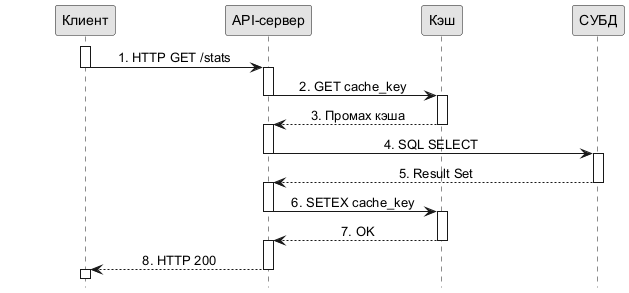
\includegraphics[width=\textwidth]{../img/cache_aside_sequence.png}
\caption{Диаграмма последовательности при паттерне Cache-Aside}
\label{fig:redis-seq}
\end{figure}

Инвалидация кэша выполняется по шаблонам ключей лидербордов, дашборда и данных команд
только для изменённого сезона, а не полным сбросом кэша: это предотвращает
одновременную инвалидацию всех ключей и снижает риск пиковой нагрузки на СУБД
при массовом промахе кэша~--- эффекта «шторма кэша», который
возникает, когда множество параллельных запросов одновременно обнаруживают
истёкший ключ и нагружают базу данных.

\section*{Вывод}

Спроектирована реляционная схема из 8~таблиц, 3~представлений и 6~ключевых индексов;
показано соответствие всех таблиц 1НФ, 2НФ и 3НФ. Бизнес-логика метрик
спроектирована в виде хранимых процедур на стороне СУБД; ограничения целостности закреплены
на уровне ограничений-проверок и триггера. Определена ролевая модель из трёх ролей
с разграничением прав на уровне таблиц, функций и представлений. Спроектировано
REST API из 22~маршрутов, организованных в пять групп и покрывающих все три
варианта использования системы. Для снижения задержки аналитических выборок
спроектировано кэширование по паттерну Cache-Aside с префиксной инвалидацией.
